


\tikzset{every picture/.style={line width=0.75pt}} %set default line width to 0.75pt        

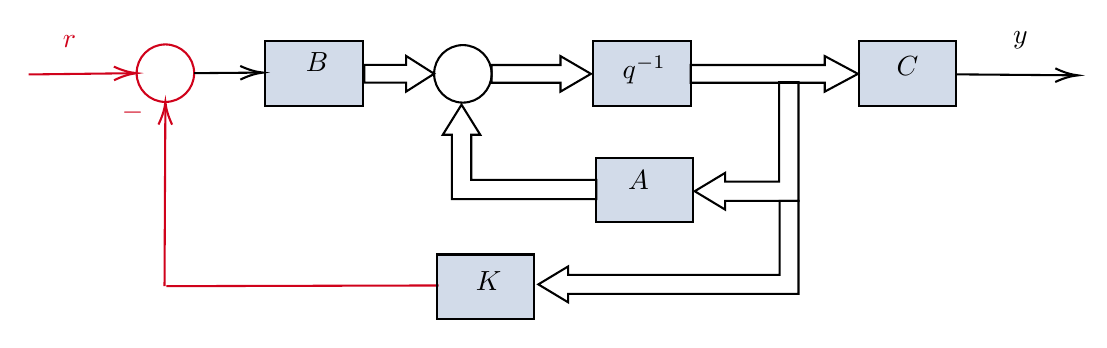
\begin{tikzpicture}[x=0.75pt,y=0.75pt,yscale=-1,xscale=1]
%uncomment if require: \path (0,300); %set diagram left start at 0, and has height of 300

%Straight Lines [id:da6568557179723491] 
\draw    (522.8,100.72) -- (579.53,101.18) ;
\draw [shift={(581.53,101.2)}, rotate = 180.47] [color={rgb, 255:red, 0; green, 0; blue, 0 }  ][line width=0.75]    (10.93,-3.29) .. controls (6.95,-1.4) and (3.31,-0.3) .. (0,0) .. controls (3.31,0.3) and (6.95,1.4) .. (10.93,3.29)   ;
%Shape: Circle [id:dp7704428899101905] 
\draw  [color={rgb, 255:red, 208; green, 2; blue, 27 }  ,draw opacity=1 ] (128,100.15) .. controls (128,92.5) and (134.2,86.3) .. (141.85,86.3) .. controls (149.5,86.3) and (155.7,92.5) .. (155.7,100.15) .. controls (155.7,107.8) and (149.5,114) .. (141.85,114) .. controls (134.2,114) and (128,107.8) .. (128,100.15) -- cycle ;
%Straight Lines [id:da5526597244895324] 
\draw [color={rgb, 255:red, 208; green, 2; blue, 27 }  ,draw opacity=1 ]   (142.27,202.77) -- (273.6,202.43) ;
%Straight Lines [id:da2893181473633277] 
\draw [color={rgb, 255:red, 208; green, 2; blue, 27 }  ,draw opacity=1 ]   (141.43,202.77) -- (141.84,116) ;
\draw [shift={(141.85,114)}, rotate = 450.27] [color={rgb, 255:red, 208; green, 2; blue, 27 }  ,draw opacity=1 ][line width=0.75]    (10.93,-3.29) .. controls (6.95,-1.4) and (3.31,-0.3) .. (0,0) .. controls (3.31,0.3) and (6.95,1.4) .. (10.93,3.29)   ;
%Straight Lines [id:da1586663427610986] 
\draw [color={rgb, 255:red, 208; green, 2; blue, 27 }  ,draw opacity=1 ]   (76,100.77) -- (126,100.17) ;
\draw [shift={(128,100.15)}, rotate = 539.3199999999999] [color={rgb, 255:red, 208; green, 2; blue, 27 }  ,draw opacity=1 ][line width=0.75]    (10.93,-3.29) .. controls (6.95,-1.4) and (3.31,-0.3) .. (0,0) .. controls (3.31,0.3) and (6.95,1.4) .. (10.93,3.29)   ;
%Shape: Rectangle [id:dp03820955712356988] 
\draw  [fill={rgb, 255:red, 158; green, 176; blue, 208 }  ,fill opacity=0.46 ] (190,84.87) -- (236.87,84.87) -- (236.87,115.97) -- (190,115.97) -- cycle ;
%Straight Lines [id:da5649251656307592] 
\draw    (155.7,100.15) -- (186.87,99.88) ;
\draw [shift={(188.87,99.87)}, rotate = 539.51] [color={rgb, 255:red, 0; green, 0; blue, 0 }  ][line width=0.75]    (10.93,-3.29) .. controls (6.95,-1.4) and (3.31,-0.3) .. (0,0) .. controls (3.31,0.3) and (6.95,1.4) .. (10.93,3.29)   ;
%Shape: Circle [id:dp6408546522042082] 
\draw  [color={rgb, 255:red, 0; green, 0; blue, 0 }  ,draw opacity=1 ] (271.33,100.48) .. controls (271.33,92.83) and (277.53,86.63) .. (285.18,86.63) .. controls (292.83,86.63) and (299.03,92.83) .. (299.03,100.48) .. controls (299.03,108.13) and (292.83,114.33) .. (285.18,114.33) .. controls (277.53,114.33) and (271.33,108.13) .. (271.33,100.48) -- cycle ;
%Right Arrow [id:dp9724398591257026] 
\draw   (237.67,96.15) -- (257.87,96.15) -- (257.87,91.87) -- (271.33,100.43) -- (257.87,109) -- (257.87,104.72) -- (237.67,104.72) -- cycle ;
%Shape: Rectangle [id:dp6319806451538068] 
\draw  [fill={rgb, 255:red, 158; green, 176; blue, 208 }  ,fill opacity=0.46 ] (272.67,187.53) -- (319.53,187.53) -- (319.53,218.63) -- (272.67,218.63) -- cycle ;
%Shape: Rectangle [id:dp2995607391602966] 
\draw  [fill={rgb, 255:red, 158; green, 176; blue, 208 }  ,fill opacity=0.46 ] (348,84.87) -- (394.87,84.87) -- (394.87,115.97) -- (348,115.97) -- cycle ;
%Right Arrow [id:dp748076149724459] 
\draw   (299.03,96.2) -- (332.2,96.2) -- (332.2,91.92) -- (346.87,100.48) -- (332.2,109.05) -- (332.2,104.77) -- (299.03,104.77) -- cycle ;
%Shape: Rectangle [id:dp7707606746542681] 
\draw  [fill={rgb, 255:red, 158; green, 176; blue, 208 }  ,fill opacity=0.46 ] (349.33,140.87) -- (396.2,140.87) -- (396.2,171.97) -- (349.33,171.97) -- cycle ;
%Bend Up Arrow [id:dp7447632849123698] 
\draw   (349.53,151.53) -- (289.21,151.53) -- (289.2,129.81) -- (293.54,129.81) -- (284.53,115.33) -- (275.52,129.81) -- (279.87,129.81) -- (279.88,160.87) -- (349.53,160.87) -- cycle ;
%Shape: Rectangle [id:dp8500153862872415] 
\draw  [fill={rgb, 255:red, 158; green, 176; blue, 208 }  ,fill opacity=0.46 ] (476,84.87) -- (522.87,84.87) -- (522.87,115.97) -- (476,115.97) -- cycle ;
%Right Arrow [id:dp13591896192936415] 
\draw   (394.87,96.2) -- (459.53,96.2) -- (459.53,91.92) -- (475.53,100.48) -- (459.53,109.05) -- (459.53,104.77) -- (394.87,104.77) -- cycle ;
%Bend Up Arrow [id:dp026003672562821434] 
\draw   (437.53,104.53) -- (437.53,152.37) -- (411.53,152.37) -- (411.53,148.2) -- (396.87,157.03) -- (411.53,165.87) -- (411.53,161.7) -- (446.87,161.7) -- (446.87,104.53) -- cycle ;
%Bend Up Arrow [id:dp017809405591459937] 
\draw   (437.75,161.7) -- (437.75,197.35) -- (335.86,197.35) -- (335.86,193.28) -- (321.53,201.91) -- (335.86,210.53) -- (335.86,206.46) -- (446.87,206.46) -- (446.87,161.7) -- cycle ;

% Text Node
\draw (290,194.4) node [anchor=north west][inner sep=0.75pt]    {$K$};
% Text Node
\draw (548.83,78.73) node [anchor=north west][inner sep=0.75pt]    {$y$};
% Text Node
\draw (91,80.4) node [anchor=north west][inner sep=0.75pt]  [color={rgb, 255:red, 208; green, 2; blue, 27 }  ,opacity=1 ]  {$r$};
% Text Node
\draw (119.33,113.4) node [anchor=north west][inner sep=0.75pt]  [color={rgb, 255:red, 208; green, 2; blue, 27 }  ,opacity=1 ]  {$-$};
% Text Node
\draw (208,88.73) node [anchor=north west][inner sep=0.75pt]    {$B$};
% Text Node
\draw (360.67,90.4) node [anchor=north west][inner sep=0.75pt]    {$q^{-1}$};
% Text Node
\draw (363.33,145.4) node [anchor=north west][inner sep=0.75pt]    {$A$};
% Text Node
\draw (492.67,90.73) node [anchor=north west][inner sep=0.75pt]    {$C$};


\end{tikzpicture}